% !TeX program = lualatex
% ALIUS Bulletin native visual reconstruction source.
% Generated from off-repo reference layout data; does not include or input a pre-existing article PDF.
\ifdefined\ALIUSIssueBuild
\else
\documentclass{article}
\usepackage[paperwidth=595.2756bp,paperheight=841.8898bp,margin=0bp]{geometry}
\usepackage{graphicx}
\usepackage{xcolor}
\usepackage{tikz}
\usepackage{iftex}
\usepackage[hidelinks]{hyperref}
\ifPDFTeX
  \usepackage[T1]{fontenc}
  \usepackage[utf8]{inputenc}
  \usepackage{textcomp}
  \usepackage{amssymb}
\else
  \usepackage{fontspec}
\fi
\pagestyle{empty}
\fi
\ifPDFTeX
  \providecommand{\ALIUSDeclareUnicodeFallbacks}{%
    \DeclareUnicodeCharacter{00AC}{\ensuremath{\neg}}%
    \DeclareUnicodeCharacter{00BE}{\ensuremath{\frac{3}{4}}}%
    \DeclareUnicodeCharacter{0101}{\=a}%
    \DeclareUnicodeCharacter{0107}{\'c}%
    \DeclareUnicodeCharacter{012B}{\=\i}%
    \DeclareUnicodeCharacter{0131}{\i}%
    \DeclareUnicodeCharacter{0142}{\l}%
    \DeclareUnicodeCharacter{015B}{\'s}%
    \DeclareUnicodeCharacter{016B}{\=u}%
    \DeclareUnicodeCharacter{025C}{q}%
    \DeclareUnicodeCharacter{0278}{t}%
    \DeclareUnicodeCharacter{02AE}{Th}%
    \DeclareUnicodeCharacter{02B0}{ff}%
    \DeclareUnicodeCharacter{02B4}{ffi}%
    \DeclareUnicodeCharacter{02BE}{ft}%
    \DeclareUnicodeCharacter{02BF}{fi}%
    \DeclareUnicodeCharacter{02C0}{fl}%
    \DeclareUnicodeCharacter{02C1}{fi}%
    \DeclareUnicodeCharacter{02D9}{Th}%
    \DeclareUnicodeCharacter{02EF}{gy}%
    \DeclareUnicodeCharacter{0394}{\ensuremath{\Delta}}%
    \DeclareUnicodeCharacter{03B2}{\ensuremath{\beta}}%
    \DeclareUnicodeCharacter{03BA}{\ensuremath{\kappa}}%
    \DeclareUnicodeCharacter{068D}{-}%
    \DeclareUnicodeCharacter{08BC}{ti}%
    \DeclareUnicodeCharacter{099E}{ti}%
    \DeclareUnicodeCharacter{1E43}{\d{m}}%
    \DeclareUnicodeCharacter{1E47}{\d{n}}%
    \DeclareUnicodeCharacter{1E63}{\d{s}}%
    \DeclareUnicodeCharacter{201C}{``}%
    \DeclareUnicodeCharacter{201D}{''}%
    \DeclareUnicodeCharacter{2018}{`}%
    \DeclareUnicodeCharacter{2019}{'}%
    \DeclareUnicodeCharacter{2260}{\ensuremath{\neq}}%
    \DeclareUnicodeCharacter{25A1}{\ensuremath{\square}}%
  }%
  \ifdefined\ALIUSIssueBuild\else\ALIUSDeclareUnicodeFallbacks\fi
  \providecommand{\ALIUSFontLatoLight}{\fontfamily{lato-LF}\fontseries{l}\selectfont}
  \providecommand{\ALIUSFontLatoRegular}{\fontfamily{lato-LF}\fontseries{m}\selectfont}
  \providecommand{\ALIUSFontLatoItalic}{\fontfamily{lato-LF}\fontseries{m}\itshape}
  \providecommand{\ALIUSFontLatoLightItalic}{\fontfamily{lato-LF}\fontseries{l}\itshape}
  \providecommand{\ALIUSFontCormorantRegular}{\fontfamily{CormorantGaramond-LF}\fontseries{m}\selectfont}
  \providecommand{\ALIUSFontCormorantLight}{\fontfamily{CormorantGaramond-LF}\fontseries{l}\selectfont}
  \providecommand{\ALIUSFontCormorantMedium}{\fontfamily{CormorantGaramond-LF}\fontseries{medium}\selectfont}
  \providecommand{\ALIUSFontCormorantBold}{\fontfamily{CormorantGaramond-LF}\fontseries{b}\selectfont}
  \providecommand{\ALIUSFontCormorantItalic}{\fontfamily{CormorantGaramond-LF}\fontseries{m}\itshape}
  \providecommand{\ALIUSFontTimes}{\fontfamily{ptm}\selectfont}
  \providecommand{\ALIUSFontCalibri}{\fontfamily{phv}\selectfont}
  \providecommand{\ALIUSFontCambria}{\fontfamily{ptm}\selectfont}
  \providecommand{\ALIUSFontSymbolFallback}{\fontfamily{ptm}\selectfont}
\else
  \providecommand{\ALIUSFontLatoLight}{\fontspec{Lato Light}}
  \providecommand{\ALIUSFontLatoRegular}{\fontspec{Lato Regular}}
  \providecommand{\ALIUSFontLatoItalic}{\fontspec{Lato Italic}}
  \providecommand{\ALIUSFontLatoLightItalic}{\fontspec{Lato Light Italic}}
  \providecommand{\ALIUSFontCormorantRegular}{\fontspec{Cormorant Garamond Regular}}
  \providecommand{\ALIUSFontCormorantLight}{\fontspec{Cormorant Garamond Light}}
  \providecommand{\ALIUSFontCormorantMedium}{\fontspec{Cormorant Garamond Medium}}
  \providecommand{\ALIUSFontCormorantBold}{\fontspec{Cormorant Garamond Bold}}
  \providecommand{\ALIUSFontCormorantItalic}{\fontspec{Cormorant Garamond Italic}}
  \providecommand{\ALIUSFontTimes}{\fontspec{Times New Roman}}
  \providecommand{\ALIUSFontCalibri}{\fontspec{Calibri}}
  \providecommand{\ALIUSFontCambria}{\fontspec{Cambria}}
  \providecommand{\ALIUSFontSymbolFallback}{\fontspec{Times New Roman}}
\fi
\providecommand{\ALIUSPullQuoteOpen}{\textquotedblleft}
\providecommand{\ALIUSPullQuoteClose}{\textquotedblright}
\providecommand{\ALIUSPullQuoteBlockAt}[4]{%
  \node[anchor=north west,inner sep=0pt,outer sep=0pt,xshift=12bp,text=ALIUSC595959,font=\ALIUSFontLatoLight\fontsize{15.000bp}{18.000bp}\selectfont\hyphenpenalty10000\exhyphenpenalty10000\relax] (ALIUSPullQuoteBody) at (#1bp,-#2bp) {\begin{tabular}{@{}c@{}}#4\end{tabular}};%
  \node[anchor=north east,inner sep=0pt,outer sep=0pt,text=ALIUSC7F7F7F,xshift=-6bp] at (ALIUSPullQuoteBody.north west) {%
    {\ALIUSFontCormorantLight\fontsize{32.000bp}{32.000bp}\selectfont\ALIUSPullQuoteOpen}%
  };%
  \node[anchor=south west,inner sep=0pt,outer sep=0pt,text=ALIUSC7F7F7F,xshift=6bp,yshift=-7bp] at (ALIUSPullQuoteBody.south east) {%
    {\ALIUSFontCormorantLight\fontsize{32.000bp}{32.000bp}\selectfont\ALIUSPullQuoteClose}%
  };%
}
\providecommand{\ALIUSNotableQuoteAt}[4]{%
  \ALIUSPullQuoteBlockAt{#1}{#2}{#3}{#4}%
}
\providecommand{\ALIUSMaybeNotableQuoteAt}[4]{%
  \if\relax\detokenize{#4}\relax\else\ALIUSNotableQuoteAt{#1}{#2}{#3}{#4}\fi%
}
\providecommand{\ALIUSRefAnchor}[1]{\hypertarget{#1}{}}
\providecommand{\ALIUSCitationLink}[2]{\hyperlink{#1}{#2}}
\definecolor{ALIUSC000000}{HTML}{000000}
\definecolor{ALIUSC1A1718}{HTML}{1A1718}
\definecolor{ALIUSC1F8135}{HTML}{1F8135}
\definecolor{ALIUSC595959}{HTML}{595959}
\definecolor{ALIUSC767171}{HTML}{767171}
\definecolor{ALIUSC7F7F7F}{HTML}{7F7F7F}
\providecommand{\ALIUSPlacedText}[6]{%
  \node[anchor=north west,inner sep=0pt,outer sep=0pt,text=#4] at (#1bp,-#2bp) {%
    \resizebox{#3bp}{!}{{#5\fontsize{#6bp}{#6bp}\selectfont #6\kern0pt}}%
  };%
}
\providecommand{\ALIUSPlacedTextContent}[7]{%
  \node[anchor=north west,inner sep=0pt,outer sep=0pt,text=#4] at (#1bp,-#2bp) {%
    \resizebox{#3bp}{!}{{#5\fontsize{#6bp}{#6bp}\selectfont #7}}%
  };%
}
\ifdefined\ALIUSIssueBuild
\else
\begin{document}
\fi
% Page 1
\thispagestyle{empty}
\noindent\begin{tikzpicture}[remember picture,overlay,x=1bp,y=1bp,shift={(current page.north west)}]
  \fill[ALIUSC767171] (76.253bp,-777.566bp) rectangle ++(443.378bp,-0.233bp);
  \fill[ALIUSC1F8135] (379.224bp,-170.224bp) rectangle ++(82.332bp,-0.233bp);
  \fill[ALIUSC1F8135] (379.224bp,-229.232bp) rectangle ++(89.095bp,-0.233bp);
  \ALIUSPlacedTextContent{84.552}{81.134}{437.075}{ALIUSC000000}{\ALIUSFontLatoRegular}{18.426}{The role of hypnosis and meditation in consciousness}
  \ALIUSPlacedTextContent{84.552}{103.292}{74.052}{ALIUSC000000}{\ALIUSFontLatoRegular}{18.426}{research}
  \ALIUSPlacedTextContent{83.016}{141.739}{118.993}{ALIUSC000000}{\ALIUSFontLatoLight}{15.627}{An interview with}
  \ALIUSPlacedTextContent{379.224}{146.819}{73.525}{ALIUSC000000}{\ALIUSFontLatoRegular}{11.662}{Zoltan Dienes}
  \ALIUSPlacedTextContent{83.016}{160.434}{113.954}{ALIUSC000000}{\ALIUSFontLatoLight}{18.426}{Zoltan Dienes}
  \ALIUSPlacedTextContent{379.224}{160.776}{84.094}{ALIUSC1F8135}{\ALIUSFontLatoLight}{8.863}{z.dienes@sussex.ac.uk}
  \ALIUSPlacedTextContent{379.224}{171.272}{105.155}{ALIUSC000000}{\ALIUSFontLatoLight}{8.863}{Departement of Psychology}
  \ALIUSPlacedTextContent{379.224}{181.767}{119.257}{ALIUSC000000}{\ALIUSFontLatoLight}{8.863}{Sussex University, Brighton, UK}
  \ALIUSPlacedTextContent{83.016}{192.311}{117.343}{ALIUSC000000}{\ALIUSFontLatoLight}{12.595}{by Jean-Rémy Martin}
  \ALIUSPlacedTextContent{379.224}{205.827}{96.557}{ALIUSC000000}{\ALIUSFontLatoRegular}{11.662}{Jean-Rémy Martin}
  \ALIUSPlacedTextContent{379.224}{219.785}{90.890}{ALIUSC1F8135}{\ALIUSFontLatoLight}{8.863}{jeanremy08@gmail.com}
  \ALIUSPlacedTextContent{379.224}{230.280}{120.296}{ALIUSC000000}{\ALIUSFontLatoLight}{8.863}{Faculty of Psychological Science}
  \ALIUSPlacedTextContent{379.224}{240.776}{54.729}{ALIUSC000000}{\ALIUSFontLatoLight}{8.863}{and Education}
  % ALIUS normalized citation panel begin
  % ALIUS normalized citation panel text: Cite as: Dienes, Z. \& Martin, J.-R. (2019). The role of hypnosis and meditation in consciousness research. An interview with Zoltan Dienes. ALIUS Bulletin,
  \fill[white] (81.516bp,-240.420bp) rectangle ++(289.208bp,-40.600bp);
  \node[anchor=north west,inner sep=0pt,outer sep=0pt,text=ALIUSC000000] at (83.016bp,-242.420bp) {\begin{minipage}{286.208bp}{\ALIUSFontLatoLight\fontsize{9.200bp}{10.700bp}\selectfont\raggedright Cite as: Dienes, Z. \& Martin, J.-R. (2019). The role of hypnosis and meditation in consciousness research. An interview with Zoltan Dienes. ALIUS Bulletin, \mbox{\textcolor{ALIUSC1F8135}{\href{https://doi.org/10.34700/jpsp-3121}{https://doi.org/10.34700/jpsp-3121}}}\par}\end{minipage}};
  % ALIUS normalized citation panel end
  \ALIUSPlacedTextContent{379.224}{251.271}{110.555}{ALIUSC000000}{\ALIUSFontLatoLight}{8.863}{Université Libre de Bruxelles,}
  \ALIUSPlacedTextContent{379.224}{261.767}{30.426}{ALIUSC000000}{\ALIUSFontLatoLight}{8.863}{Belgium}
  \ALIUSPlacedTextContent{77.652}{310.836}{45.118}{ALIUSC000000}{\ALIUSFontLatoLight}{11.547}{Abstract}
  \ALIUSPlacedTextContent{77.652}{330.607}{442.780}{ALIUSC000000}{\ALIUSFontLatoLight}{11.662}{In this interview, Zoltan Dienes (Brighton, UK), specialist in consciousness studies, answers}
  \ALIUSPlacedTextContent{77.652}{344.601}{442.774}{ALIUSC000000}{\ALIUSFontLatoLight}{11.662}{questions related to hypnosis and meditation: Why are hypnosis and mindfulness}
  \ALIUSPlacedTextContent{77.652}{358.595}{442.785}{ALIUSC000000}{\ALIUSFontLatoLight}{11.662}{interesting topics for the study of consciousness? Is the notion of altered state of}
  \ALIUSPlacedTextContent{77.652}{372.589}{442.784}{ALIUSC000000}{\ALIUSFontLatoLight}{11.662}{consciousness a useful notion in the context of hypnosis and mindfulness? What do we}
  \ALIUSPlacedTextContent{77.652}{386.583}{442.773}{ALIUSC000000}{\ALIUSFontLatoLight}{11.662}{know about the neurocognitive mechanisms sustaining the action of hypnosis and}
  \ALIUSPlacedTextContent{77.652}{400.577}{442.779}{ALIUSC000000}{\ALIUSFontLatoLight}{11.662}{mindfulness? There is a long tradition of using hypnosis clinically, particularly as an}
  \ALIUSPlacedTextContent{77.652}{414.572}{442.777}{ALIUSC000000}{\ALIUSFontLatoLight}{11.662}{analgesic method; might mindfulness and hypnosis work in the same way? Building on his}
  \ALIUSPlacedTextContent{77.652}{428.566}{442.774}{ALIUSC000000}{\ALIUSFontLatoLight}{11.662}{empirical and theoretical research on hypnosis and meditation, Zoltan Dienes gives us his}
  \ALIUSPlacedTextContent{77.652}{442.560}{442.777}{ALIUSC000000}{\ALIUSFontLatoLight}{11.662}{answers. Hypnosis and meditation are postulated to engage metacognitive processes,}
  \ALIUSPlacedTextContent{77.652}{456.554}{123.618}{ALIUSC000000}{\ALIUSFontLatoLight}{11.662}{though in opposite ways.}
  \ALIUSPlacedTextContent{119.909}{488.028}{223.270}{ALIUSC000000}{\ALIUSFontLatoLightItalic}{10.729}{~consciousness, hypnosis, meditation, metacognition.}
  \ALIUSPlacedTextContent{77.652}{488.073}{42.252}{ALIUSC000000}{\ALIUSFontLatoLightItalic}{10.623}{keywords:}
  \ALIUSPlacedTextContent{77.652}{518.600}{433.642}{ALIUSC1F8135}{\ALIUSFontLatoLight}{12.128}{Why are hypnosis and mindfulness interesting topics for the study of consciousness?}
  \ALIUSPlacedTextContent{77.652}{544.660}{443.578}{ALIUSC000000}{\ALIUSFontCormorantMedium}{13.528}{Hypnotic response involves distortions in consciousness:  hallucinations, delusions,}
  \ALIUSPlacedTextContent{77.652}{561.219}{443.656}{ALIUSC000000}{\ALIUSFontCormorantMedium}{13.528}{and altered experiences of agency. Thus, the fundamental facts to be explained in}
  \ALIUSPlacedTextContent{77.652}{577.779}{443.698}{ALIUSC000000}{\ALIUSFontCormorantMedium}{13.528}{hypnosis involve the nature of conscious experience. It may be these different}
  \ALIUSPlacedTextContent{77.652}{594.105}{443.685}{ALIUSC000000}{\ALIUSFontCormorantMedium}{13.528}{experiences rely on a single distortion in conscious experience: That of non-volition.}
  \ALIUSPlacedTextContent{77.652}{610.665}{443.750}{ALIUSC000000}{\ALIUSFontCormorantMedium}{13.528}{In fact, Weitzenhoffer (1978) defined the “classic suggestion effect” as the experience}
  \ALIUSPlacedTextContent{77.652}{627.225}{443.683}{ALIUSC000000}{\ALIUSFontCormorantMedium}{13.528}{of a response being non-volitional. For example, if we take a suggested motor}
  \ALIUSPlacedTextContent{77.652}{643.551}{443.629}{ALIUSC000000}{\ALIUSFontCormorantMedium}{13.528}{response, like the arm rising in the air by itself, in several prominent theories of}
  \ALIUSPlacedTextContent{77.652}{660.111}{443.592}{ALIUSC000000}{\ALIUSFontCormorantMedium}{13.528}{hypnosis (like those of either Hilgard or Spanos) the person does intend for the arm}
  \ALIUSPlacedTextContent{77.652}{676.437}{443.663}{ALIUSC000000}{\ALIUSFontCormorantMedium}{13.528}{to rise; but the experience is that they did not intend it. So, in these accounts,}
  \ALIUSPlacedTextContent{77.652}{692.997}{443.631}{ALIUSC000000}{\ALIUSFontCormorantMedium}{13.528}{hypnotic response involves an illusion of involuntariness; in fact, in these accounts}
  \ALIUSPlacedTextContent{77.652}{709.556}{443.624}{ALIUSC000000}{\ALIUSFontCormorantMedium}{13.528}{it is precisely that illusion that makes a response hypnotic. The illusion presents a}
  \ALIUSPlacedTextContent{77.652}{725.883}{443.684}{ALIUSC000000}{\ALIUSFontCormorantMedium}{13.528}{unique window into the nature of experienced volition for consciousness}
  \ALIUSPlacedTextContent{77.652}{742.443}{443.597}{ALIUSC000000}{\ALIUSFontCormorantMedium}{13.528}{researchers. This illusion may give rise not only to feelings of involuntariness during}
  \ALIUSPlacedTextContent{77.652}{783.303}{117.883}{ALIUSC767171}{\ALIUSFontLatoLight}{10.729}{ALIUS Bulletin n°3 (2019)}
  \ALIUSPlacedTextContent{402.025}{783.303}{116.144}{ALIUSC767171}{\ALIUSFontLatoLight}{10.729}{aliusresearch.org/bulletin}
\end{tikzpicture}
\null
\newpage
% Page 2
\thispagestyle{empty}
\noindent\begin{tikzpicture}[remember picture,overlay,x=1bp,y=1bp,shift={(current page.north west)}]
  \fill[ALIUSC767171] (76.253bp,-65.268bp) rectangle ++(443.378bp,-0.233bp);
  \fill[ALIUSC767171] (76.253bp,-777.332bp) rectangle ++(443.378bp,-0.466bp);
  \ALIUSPlacedTextContent{77.652}{46.516}{354.220}{ALIUSC767171}{\ALIUSFontLatoLight}{10.729}{Zoltan Dienes - The role of hypnosis and meditation in consciousness research}
  \ALIUSPlacedTextContent{505.773}{46.516}{14.471}{ALIUSC767171}{\ALIUSFontLatoLight}{10.729}{28}
  \ALIUSPlacedTextContent{77.652}{81.223}{443.527}{ALIUSC000000}{\ALIUSFontCormorantMedium}{13.528}{motor responses but also to the other distortions of consciousness just mentioned,}
  \ALIUSPlacedTextContent{77.652}{97.550}{443.693}{ALIUSC000000}{\ALIUSFontCormorantMedium}{13.528}{namely, hallucinations and delusions. For example, consider a suggestion that one}
  \ALIUSPlacedTextContent{77.652}{114.109}{443.682}{ALIUSC000000}{\ALIUSFontCormorantMedium}{13.528}{will see an elephant.  If one intends to imagine the elephant, but is unaware of that}
  \ALIUSPlacedTextContent{77.652}{130.669}{443.580}{ALIUSC000000}{\ALIUSFontCormorantMedium}{13.528}{intention, the imagination may be experienced as a perception: A hallucination.  Or}
  \ALIUSPlacedTextContent{77.652}{146.995}{443.643}{ALIUSC000000}{\ALIUSFontCormorantMedium}{13.528}{consider a suggestion that one has the opposite sex to one’s actual sex.  If one intends}
  \ALIUSPlacedTextContent{77.652}{163.555}{443.635}{ALIUSC000000}{\ALIUSFontCormorantMedium}{13.528}{to engage in pretence, but is unaware of that intention, the pretence may be}
  \ALIUSPlacedTextContent{77.652}{180.115}{443.689}{ALIUSC000000}{\ALIUSFontCormorantMedium}{13.528}{experienced as a belief: A delusion. That in any case, is my take on hypnotic response}
  \ALIUSPlacedTextContent{77.652}{196.441}{443.610}{ALIUSC000000}{\ALIUSFontCormorantMedium}{13.528}{(e.g. \ALIUSCitationLink{aliusref-dienes-martin-dienes-perner-2007}{Dienes \& Perner, 2007}). This view of hypnosis is naturally related to a key}
  \ALIUSPlacedTextContent{77.652}{213.001}{443.690}{ALIUSC000000}{\ALIUSFontCormorantMedium}{13.528}{approach to understanding consciousness: Higher order theories, like that of}
  \ALIUSPlacedTextContent{77.652}{229.560}{443.632}{ALIUSC000000}{\ALIUSFontCormorantMedium}{13.528}{Rosenthal (2005). According to higher order theories, a mental state being conscious}
  \ALIUSPlacedTextContent{77.652}{246.120}{222.233}{ALIUSC000000}{\ALIUSFontCormorantMedium}{13.528}{requires one be aware of that mental state}
  \ALIUSPlacedTextContent{308.011}{246.120}{128.414}{ALIUSC000000}{\ALIUSFontCormorantMedium}{13.528}{by a higher order state.}
  \ALIUSPlacedTextContent{299.945}{249.568}{8.131}{ALIUSC000000}{\ALIUSFontCormorantMedium}{9.796}{—}
  \ALIUSPlacedTextContent{77.652}{274.108}{443.673}{ALIUSC000000}{\ALIUSFontCormorantMedium}{13.528}{If the essence of hypnotic response is intending while forming the higher order}
  \ALIUSPlacedTextContent{77.652}{290.668}{443.729}{ALIUSC000000}{\ALIUSFontCormorantMedium}{13.528}{thought that one is not intending, then hypnosis is naturally linked to one of the}
  \ALIUSPlacedTextContent{77.652}{306.994}{443.570}{ALIUSC000000}{\ALIUSFontCormorantMedium}{13.528}{major approaches to understanding consciousness: The illusion of involuntariness}
  \ALIUSPlacedTextContent{77.652}{323.554}{443.753}{ALIUSC000000}{\ALIUSFontCormorantMedium}{13.528}{comes about by inaccurate higher order thoughts. Even if one didn’t subscribe to}
  \ALIUSPlacedTextContent{77.652}{339.880}{443.654}{ALIUSC000000}{\ALIUSFontCormorantMedium}{13.528}{higher order theory as an account of a mental state being conscious, one would}
  \ALIUSPlacedTextContent{77.652}{356.440}{443.698}{ALIUSC000000}{\ALIUSFontCormorantMedium}{13.528}{surely subscribe to the view that having higher order thoughts is an interesting form}
  \ALIUSPlacedTextContent{77.652}{372.999}{443.679}{ALIUSC000000}{\ALIUSFontCormorantMedium}{13.528}{of consciousness.  So I think hypnosis should play a more prominent role in}
  \ALIUSPlacedTextContent{77.652}{389.559}{238.167}{ALIUSC000000}{\ALIUSFontCormorantMedium}{13.528}{consciousness science than it currently does!}
  \ALIUSPlacedTextContent{124.936}{434.902}{24.676}{ALIUSC7F7F7F}{\ALIUSFontCormorantLight}{46.647}{\ALIUSPullQuoteOpen}
  \ALIUSPlacedTextContent{142.936}{434.902}{309.127}{ALIUSC595959}{\ALIUSFontLatoLight}{14.694}{I think hypnosis should play a more prominent role}
  \ALIUSPlacedTextContent{456.063}{452.395}{13.761}{ALIUSC7F7F7F}{\ALIUSFontCormorantLight}{46.647}{\ALIUSPullQuoteClose}
  \ALIUSPlacedTextContent{149.249}{452.395}{296.503}{ALIUSC595959}{\ALIUSFontLatoLight}{14.694}{in consciousness science than it currently does!}
  \ALIUSPlacedTextContent{77.652}{500.345}{443.688}{ALIUSC000000}{\ALIUSFontCormorantMedium}{13.528}{Just as hypnosis may essentially be a meta-cognitive phenomenon, so is mindfulness.}
  \ALIUSPlacedTextContent{77.652}{516.672}{443.648}{ALIUSC000000}{\ALIUSFontCormorantMedium}{13.528}{Mindfulness is a matter of having certain sorts of higher order states. One Pali sutta}
  \ALIUSPlacedTextContent{77.652}{533.231}{443.659}{ALIUSC000000}{\ALIUSFontCormorantMedium}{13.528}{compares mindfulness to a surgeon’s probe that is used to explore tissue so that the}
  \ALIUSPlacedTextContent{77.652}{549.791}{443.693}{ALIUSC000000}{\ALIUSFontCormorantMedium}{13.528}{surgeon knows how to use the knife. A probe is used to show things as they are so}
  \ALIUSPlacedTextContent{77.652}{566.117}{443.847}{ALIUSC000000}{\ALIUSFontCormorantMedium}{13.528}{that one can act appropriately. Thus, one aspect of mindfulness is accurate}
  \ALIUSPlacedTextContent{77.652}{582.677}{443.716}{ALIUSC000000}{\ALIUSFontCormorantMedium}{13.528}{awareness of mental states.  In this way, there is a tension between being mindful}
  \ALIUSPlacedTextContent{77.652}{599.237}{443.692}{ALIUSC000000}{\ALIUSFontCormorantMedium}{13.528}{and hypnotic responding, because my view of hypnotic response is that it is a}
  \ALIUSPlacedTextContent{77.652}{615.563}{443.765}{ALIUSC000000}{\ALIUSFontCormorantMedium}{13.528}{response in which one is (strategically) not mindful of the corresponding intention,}
  \ALIUSPlacedTextContent{77.652}{632.123}{443.634}{ALIUSC000000}{\ALIUSFontCormorantMedium}{13.528}{as I discussed above. Thus, mindfulness also intrinsically relates to a major theory of}
  \ALIUSPlacedTextContent{77.652}{648.682}{233.228}{ALIUSC000000}{\ALIUSFontCormorantMedium}{13.528}{consciousness, namely higher order theory.}
  \ALIUSPlacedTextContent{146.970}{694.259}{24.676}{ALIUSC7F7F7F}{\ALIUSFontCormorantLight}{46.647}{\ALIUSPullQuoteOpen}
  \ALIUSPlacedTextContent{164.970}{694.259}{265.059}{ALIUSC595959}{\ALIUSFontLatoLight}{14.694}{Just as hypnosis may essentially be a meta-}
  \ALIUSPlacedTextContent{434.029}{711.751}{13.761}{ALIUSC7F7F7F}{\ALIUSFontCormorantLight}{46.647}{\ALIUSPullQuoteClose}
  \ALIUSPlacedTextContent{167.801}{711.751}{259.398}{ALIUSC595959}{\ALIUSFontLatoLight}{14.694}{cognitive phenomenon, so is mindfulness.}
  \ALIUSPlacedTextContent{77.652}{783.303}{117.883}{ALIUSC767171}{\ALIUSFontLatoLight}{10.729}{ALIUS Bulletin n°3 (2019)}
  \ALIUSPlacedTextContent{402.025}{783.303}{116.144}{ALIUSC767171}{\ALIUSFontLatoLight}{10.729}{aliusresearch.org/bulletin}
\end{tikzpicture}
\null
\newpage
% Page 3
\thispagestyle{empty}
\noindent\begin{tikzpicture}[remember picture,overlay,x=1bp,y=1bp,shift={(current page.north west)}]
  \fill[ALIUSC767171] (76.253bp,-65.268bp) rectangle ++(443.378bp,-0.233bp);
  \fill[ALIUSC767171] (76.253bp,-777.332bp) rectangle ++(443.378bp,-0.466bp);
  \ALIUSPlacedTextContent{77.652}{46.516}{354.220}{ALIUSC767171}{\ALIUSFontLatoLight}{10.729}{Zoltan Dienes - The role of hypnosis and meditation in consciousness research}
  \ALIUSPlacedTextContent{505.773}{46.516}{14.471}{ALIUSC767171}{\ALIUSFontLatoLight}{10.729}{29}
  \ALIUSPlacedTextContent{77.652}{81.223}{443.735}{ALIUSC000000}{\ALIUSFontCormorantMedium}{13.528}{Buddhist mindfulness also involves as its first foundation training awareness of one’s}
  \ALIUSPlacedTextContent{77.652}{97.550}{443.616}{ALIUSC000000}{\ALIUSFontCormorantMedium}{13.528}{body, including proprioception and interoception. Why was this regarded as a}
  \ALIUSPlacedTextContent{77.652}{114.109}{443.635}{ALIUSC000000}{\ALIUSFontCormorantMedium}{13.528}{practice conducive to flourishing? Part of the answer to possible beneficial effects}
  \ALIUSPlacedTextContent{77.652}{130.669}{443.598}{ALIUSC000000}{\ALIUSFontCormorantMedium}{13.528}{may relate to current theories in consciousness science, especially those using the}
  \ALIUSPlacedTextContent{77.652}{146.995}{443.621}{ALIUSC000000}{\ALIUSFontCormorantMedium}{13.528}{predictive processing framework, placing importance on interoceptive awareness in,}
  \ALIUSPlacedTextContent{77.652}{163.555}{443.760}{ALIUSC000000}{\ALIUSFontCormorantMedium}{13.528}{for example, constituting emotion (Seth and Critchley, 2016).  But how this works}
  \ALIUSPlacedTextContent{77.652}{180.115}{443.669}{ALIUSC000000}{\ALIUSFontCormorantMedium}{13.528}{has yet to be spelled out. One phenomenon provides an interesting challenge to}
  \ALIUSPlacedTextContent{77.652}{196.441}{443.597}{ALIUSC000000}{\ALIUSFontCormorantMedium}{13.528}{predictive processing theories (to be discussed below): Attention to action in a}
  \ALIUSPlacedTextContent{77.652}{213.001}{443.687}{ALIUSC000000}{\ALIUSFontCormorantMedium}{13.528}{deliberate way may decrease the sense it is volitional (a point Martin \& Pacherie,}
  \ALIUSPlacedTextContent{77.652}{229.560}{443.743}{ALIUSC000000}{\ALIUSFontCormorantMedium}{13.528}{2019, use as a predictive processing theory of hypnosis), but attention to breath (as}
  \ALIUSPlacedTextContent{77.652}{245.887}{443.553}{ALIUSC000000}{\ALIUSFontCormorantMedium}{13.528}{in many types of meditation) increases the sense of voluntary control. We return to}
  \ALIUSPlacedTextContent{77.652}{262.446}{88.864}{ALIUSC000000}{\ALIUSFontCormorantMedium}{13.528}{this issue below.}
  \ALIUSPlacedTextContent{77.652}{290.497}{166.894}{ALIUSC1F8135}{\ALIUSFontLatoLight}{12.128}{Do you think that the notion of}
  \ALIUSPlacedTextContent{245.685}{290.497}{145.929}{ALIUSC1F8135}{\ALIUSFontLatoLightItalic}{12.128}{~altered state of consciousness}
  \ALIUSPlacedTextContent{391.633}{290.497}{128.901}{ALIUSC1F8135}{\ALIUSFontLatoLight}{12.128}{~is a useful notion in the}
  \ALIUSPlacedTextContent{77.652}{305.191}{197.447}{ALIUSC1F8135}{\ALIUSFontLatoLight}{12.128}{context of hypnosis and mindfulness?}
  \ALIUSPlacedTextContent{77.652}{331.484}{443.742}{ALIUSC000000}{\ALIUSFontCormorantMedium}{13.528}{It is a useful concept in both cases simply because it is part of phenomena claimed}
  \ALIUSPlacedTextContent{77.652}{347.810}{443.760}{ALIUSC000000}{\ALIUSFontCormorantMedium}{13.528}{to exist; and thus, the nature of any putative altered state is something we need to}
  \ALIUSPlacedTextContent{77.652}{364.370}{443.702}{ALIUSC000000}{\ALIUSFontCormorantMedium}{13.528}{settle one way or the other. An altered state of consciousness means there is some}
  \ALIUSPlacedTextContent{77.652}{380.696}{443.796}{ALIUSC000000}{\ALIUSFontCormorantMedium}{13.528}{systematic change in how consciousness as a whole functions. For example, being in}
  \ALIUSPlacedTextContent{77.652}{397.256}{443.684}{ALIUSC000000}{\ALIUSFontCormorantMedium}{13.528}{one emotion rather than another involves altering the state of consciousness,}
  \ALIUSPlacedTextContent{77.652}{413.815}{443.594}{ALIUSC000000}{\ALIUSFontCormorantMedium}{13.528}{because there are systematic changes in how attention works, in motivation, and so}
  \ALIUSPlacedTextContent{77.652}{430.142}{443.785}{ALIUSC000000}{\ALIUSFontCormorantMedium}{13.528}{on. The altered state often involves facilitating or inhibiting specific cognitive}
  \ALIUSPlacedTextContent{77.652}{446.701}{443.685}{ALIUSC000000}{\ALIUSFontCormorantMedium}{13.528}{actions; maybe for example, being happy facilitates broad attentional focus, use of}
  \ALIUSPlacedTextContent{77.652}{463.261}{395.304}{ALIUSC000000}{\ALIUSFontCormorantMedium}{13.528}{stereotypes and so on. So interesting altered states have causal properties.}
  \ALIUSPlacedTextContent{142.120}{508.838}{24.676}{ALIUSC7F7F7F}{\ALIUSFontCormorantLight}{46.647}{\ALIUSPullQuoteOpen}
  \ALIUSPlacedTextContent{160.120}{508.838}{274.760}{ALIUSC595959}{\ALIUSFontLatoLight}{14.694}{The nature of any putative altered state in}
  \ALIUSPlacedTextContent{160.186}{526.330}{274.628}{ALIUSC595959}{\ALIUSFontLatoLight}{14.694}{hypnosis or meditation is something we need}
  \ALIUSPlacedTextContent{438.880}{543.822}{13.761}{ALIUSC7F7F7F}{\ALIUSFontCormorantLight}{46.647}{\ALIUSPullQuoteClose}
  \ALIUSPlacedTextContent{202.462}{543.822}{190.076}{ALIUSC595959}{\ALIUSFontLatoLight}{14.694}{to settle one way or the other.}
  \ALIUSPlacedTextContent{77.652}{587.575}{443.596}{ALIUSC000000}{\ALIUSFontCormorantMedium}{13.528}{Now, historically there have been two phenomena claimed to define hypnosis: First,}
  \ALIUSPlacedTextContent{77.652}{603.901}{443.671}{ALIUSC000000}{\ALIUSFontCormorantMedium}{13.528}{there is the claim that there are hypnotic responses, namely suggested alterations in}
  \ALIUSPlacedTextContent{77.652}{620.461}{443.621}{ALIUSC000000}{\ALIUSFontCormorantMedium}{13.528}{conscious experience, as I discussed above. This claim I take to be solid. Second,}
  \ALIUSPlacedTextContent{77.652}{637.021}{443.749}{ALIUSC000000}{\ALIUSFontCormorantMedium}{13.528}{there is the claim that hypnosis is an altered state of consciousness that facilitates}
  \ALIUSPlacedTextContent{77.652}{653.347}{443.686}{ALIUSC000000}{\ALIUSFontCormorantMedium}{13.528}{such hypnotic response. There is still debate about this. Highly hypnotisable people}
  \ALIUSPlacedTextContent{77.652}{669.907}{443.648}{ALIUSC000000}{\ALIUSFontCormorantMedium}{13.528}{do experience broad phenomenological changes when “hypnotized” (Pekala \&}
  \ALIUSPlacedTextContent{77.652}{686.466}{443.713}{ALIUSC000000}{\ALIUSFontCormorantMedium}{13.528}{Kumar, 2007).  One explanation is that these experiences are suggested effects; in}
  \ALIUSPlacedTextContent{77.652}{702.793}{443.627}{ALIUSC000000}{\ALIUSFontCormorantMedium}{13.528}{other words, this phenomenon is just a specific case of the first phenomenon, namely}
  \ALIUSPlacedTextContent{77.652}{719.352}{443.555}{ALIUSC000000}{\ALIUSFontCormorantMedium}{13.528}{hypnotic response. If the experience of an altered state is just another hypnotic}
  \ALIUSPlacedTextContent{77.652}{735.912}{443.656}{ALIUSC000000}{\ALIUSFontCormorantMedium}{13.528}{response, then the altered state would have no causal role in facilitating response to}
  \ALIUSPlacedTextContent{77.652}{783.303}{117.883}{ALIUSC767171}{\ALIUSFontLatoLight}{10.729}{ALIUS Bulletin n°3 (2019)}
  \ALIUSPlacedTextContent{402.025}{783.303}{116.144}{ALIUSC767171}{\ALIUSFontLatoLight}{10.729}{aliusresearch.org/bulletin}
\end{tikzpicture}
\null
\newpage
% Page 4
\thispagestyle{empty}
\noindent
\begin{tikzpicture}[remember picture,overlay,x=1bp,y=1bp,shift={(current page.north west)}]
  \fill[ALIUSC767171] (76.253bp,-65.268bp) rectangle ++(443.378bp,-0.233bp);
  \fill[ALIUSC767171] (76.253bp,-777.332bp) rectangle ++(443.378bp,-0.466bp);
  \ALIUSPlacedTextContent{77.652}{46.516}{354.220}{ALIUSC767171}{\ALIUSFontLatoLight}{10.729}{Zoltan Dienes - The role of hypnosis and meditation in consciousness research}
  \ALIUSPlacedTextContent{505.773}{46.516}{14.471}{ALIUSC767171}{\ALIUSFontLatoLight}{10.729}{30}
  \ALIUSPlacedTextContent{77.652}{81.223}{443.589}{ALIUSC000000}{\ALIUSFontCormorantMedium}{13.528}{further suggestions. In fact, hypnotic inductions do increase the rate of hypnotic}
  \ALIUSPlacedTextContent{77.652}{97.550}{443.610}{ALIUSC000000}{\ALIUSFontCormorantMedium}{13.528}{response. But on average by a tiny amount. They also increase the expectation of}
  \ALIUSPlacedTextContent{77.652}{114.109}{443.691}{ALIUSC000000}{\ALIUSFontCormorantMedium}{13.528}{successfully responding. And maybe that is all there is to it: Increase expectations or}
  \ALIUSPlacedTextContent{77.652}{130.669}{443.564}{ALIUSC000000}{\ALIUSFontCormorantMedium}{13.528}{motivation slightly and you increase response a bit, without the need to postulate a}
  \ALIUSPlacedTextContent{77.652}{146.995}{443.750}{ALIUSC000000}{\ALIUSFontCormorantMedium}{13.528}{special causal altered state (Braffman \& Kirsch, 1999). I personally side with this way}
  \ALIUSPlacedTextContent{77.652}{163.555}{443.664}{ALIUSC000000}{\ALIUSFontCormorantMedium}{13.528}{of looking at the role of altered states in hypnosis because it is simplest. The one}
  \ALIUSPlacedTextContent{77.652}{180.115}{443.626}{ALIUSC000000}{\ALIUSFontCormorantMedium}{13.528}{case I know of where an induction massively increased hypnotic response is the}
  \ALIUSPlacedTextContent{77.652}{196.441}{443.683}{ALIUSC000000}{\ALIUSFontCormorantMedium}{13.528}{suggested delusional belief that one’s reflection in the mirror is a stranger; Connors}
  \ALIUSPlacedTextContent{77.652}{213.001}{443.706}{ALIUSC000000}{\ALIUSFontCormorantMedium}{13.528}{et al. (2012) found a response rate of 70\% after an induction and 22\% without. This}
  \ALIUSPlacedTextContent{77.652}{229.560}{443.478}{ALIUSC000000}{\ALIUSFontCormorantMedium}{13.528}{may be a causal effect of induction reducing critical thinking; or it may be due to}
  \ALIUSPlacedTextContent{77.652}{246.120}{72.347}{ALIUSC000000}{\ALIUSFontCormorantMedium}{13.528}{expectations.}
  \ALIUSPlacedTextContent{77.652}{274.108}{443.710}{ALIUSC000000}{\ALIUSFontCormorantMedium}{13.528}{Meditation has of course also been claimed to be an altered state. Historically, in}
  \ALIUSPlacedTextContent{77.652}{290.668}{443.653}{ALIUSC000000}{\ALIUSFontCormorantMedium}{13.528}{the experimental academic literature, these claims have related to the sort of}
  \ALIUSPlacedTextContent{77.652}{306.994}{443.502}{ALIUSC000000}{\ALIUSFontCormorantMedium}{13.528}{meditation that aims to promote deep absorption in a simple mental state, so the}
  \ALIUSPlacedTextContent{77.652}{323.554}{443.624}{ALIUSC000000}{\ALIUSFontCormorantMedium}{13.528}{normal complexity of mental life falls away. While such concentration involves}
  \ALIUSPlacedTextContent{77.652}{339.880}{443.676}{ALIUSC000000}{\ALIUSFontCormorantMedium}{13.528}{mindfulness, mindfulness does not necessitate such concentration. Indeed, the aim}
  \ALIUSPlacedTextContent{77.652}{356.440}{443.613}{ALIUSC000000}{\ALIUSFontCormorantMedium}{13.528}{of much mindfulness meditation is to maintain a requisite level of richness in order}
  \ALIUSPlacedTextContent{77.652}{372.999}{443.870}{ALIUSC000000}{\ALIUSFontCormorantMedium}{13.528}{to be aware of what is actually going on in one’s mental life, and to do so to an extent}
  \ALIUSPlacedTextContent{77.652}{389.326}{443.714}{ALIUSC000000}{\ALIUSFontCormorantMedium}{13.528}{that mindfulness generalizes to everyday life. The Buddhist claim is that one would}
  \ALIUSPlacedTextContent{77.652}{405.885}{443.710}{ALIUSC000000}{\ALIUSFontCormorantMedium}{13.528}{then be in a globally different state (see \ALIUSCitationLink{aliusref-dienes-martin-boyle-2015}{Boyle, 2015}, for interviews with meditation}
  \ALIUSPlacedTextContent{77.652}{422.445}{443.727}{ALIUSC000000}{\ALIUSFontCormorantMedium}{13.528}{teachers about their experiences along these lines).  Further, the Buddhist claim is}
  \ALIUSPlacedTextContent{77.652}{438.771}{443.700}{ALIUSC000000}{\ALIUSFontCormorantMedium}{13.528}{that when one is fully mindful of one’s mental states there is an awareness that no}
  \ALIUSPlacedTextContent{77.652}{455.331}{443.567}{ALIUSC000000}{\ALIUSFontCormorantMedium}{13.528}{“I” exists beyond the mental states themselves and their causal flow. If one felt this}
  \ALIUSPlacedTextContent{77.652}{471.891}{443.675}{ALIUSC000000}{\ALIUSFontCormorantMedium}{13.528}{experientially, it would be an altered state of consciousness (Berkovich-Ohana et al.,}
  \ALIUSPlacedTextContent{77.652}{488.217}{443.680}{ALIUSC000000}{\ALIUSFontCormorantMedium}{13.528}{2013). My own research says little about this; but whatever altered state is involved}
  \ALIUSPlacedTextContent{77.652}{504.777}{443.648}{ALIUSC000000}{\ALIUSFontCormorantMedium}{13.528}{with mindfulness, it would be, for the reasons discussed above, a rather different}
  \ALIUSPlacedTextContent{77.652}{521.336}{207.555}{ALIUSC000000}{\ALIUSFontCormorantMedium}{13.528}{one from that involved with hypnosis.}
  \ALIUSPlacedTextContent{77.652}{549.324}{443.694}{ALIUSC000000}{\ALIUSFontCormorantMedium}{13.528}{While I think hypnosis and mindfulness are constitutively different, that is not to}
  \ALIUSPlacedTextContent{77.652}{565.884}{443.666}{ALIUSC000000}{\ALIUSFontCormorantMedium}{13.528}{say phenomena that come under the heading of each in practice are really different.}
  \ALIUSPlacedTextContent{77.652}{582.211}{443.594}{ALIUSC000000}{\ALIUSFontCormorantMedium}{13.528}{That is, I think it is an open question how much of the altered states described as}
  \ALIUSPlacedTextContent{77.652}{598.770}{443.700}{ALIUSC000000}{\ALIUSFontCormorantMedium}{13.528}{arising in meditation may actually be suggested phenomena experienced}
  \ALIUSPlacedTextContent{77.652}{615.330}{65.837}{ALIUSC000000}{\ALIUSFontCormorantMedium}{13.528}{hypnotically}
  \ALIUSPlacedTextContent{151.580}{615.330}{369.769}{ALIUSC000000}{\ALIUSFontCormorantMedium}{13.528}{so are not involving mindfulness fully, but rather hypnosis (Dienes et}
  \ALIUSPlacedTextContent{143.514}{618.778}{8.131}{ALIUSC000000}{\ALIUSFontCormorantMedium}{9.796}{—}
  \ALIUSPlacedTextContent{77.652}{631.656}{443.623}{ALIUSC000000}{\ALIUSFontCormorantMedium}{13.528}{al., 2016). For example, in absorption meditation one goes through a set of prescribed}
  \ALIUSPlacedTextContent{77.652}{648.216}{443.713}{ALIUSC000000}{\ALIUSFontCormorantMedium}{13.528}{stages of experience, an increasing depth of an altered state, as for example bodily}
  \ALIUSPlacedTextContent{77.652}{664.776}{425.372}{ALIUSC000000}{\ALIUSFontCormorantMedium}{13.528}{pleasures arise and fade. I plan to investigate how much this could be suggested.}
  \ALIUSPlacedTextContent{77.652}{692.826}{443.055}{ALIUSC1F8135}{\ALIUSFontLatoLight}{12.128}{Do we have an idea of the neurocognitive mechanisms sustaining the action of hypnosis}
  \ALIUSPlacedTextContent{77.652}{707.520}{92.991}{ALIUSC1F8135}{\ALIUSFontLatoLight}{12.128}{and mindfulness?}
  \ALIUSPlacedTextContent{77.652}{783.303}{117.883}{ALIUSC767171}{\ALIUSFontLatoLight}{10.729}{ALIUS Bulletin n°3 (2019)}
  \ALIUSPlacedTextContent{402.025}{783.303}{116.144}{ALIUSC767171}{\ALIUSFontLatoLight}{10.729}{aliusresearch.org/bulletin}
\end{tikzpicture}
\null
\newpage
% Page 5
\thispagestyle{empty}
\noindent\begin{tikzpicture}[remember picture,overlay,x=1bp,y=1bp,shift={(current page.north west)}]
  \fill[ALIUSC767171] (76.253bp,-65.268bp) rectangle ++(443.378bp,-0.233bp);
  \fill[ALIUSC767171] (76.253bp,-777.332bp) rectangle ++(443.378bp,-0.466bp);
  \fill[ALIUSC000000] (77.652bp,-711.327bp) rectangle ++(139.941bp,-0.466bp);
  \ALIUSPlacedTextContent{77.652}{46.516}{354.220}{ALIUSC767171}{\ALIUSFontLatoLight}{10.729}{Zoltan Dienes - The role of hypnosis and meditation in consciousness research}
  \ALIUSPlacedTextContent{505.773}{46.516}{14.471}{ALIUSC767171}{\ALIUSFontLatoLight}{10.729}{31}
  \ALIUSPlacedTextContent{77.652}{81.223}{443.687}{ALIUSC000000}{\ALIUSFontCormorantMedium}{13.528}{First we need a theory at the cognitive level of each phenomenon, then we can start}
  \ALIUSPlacedTextContent{77.652}{97.550}{443.729}{ALIUSC000000}{\ALIUSFontCormorantMedium}{13.528}{to relate the theoretical processes to the neural basis. One starting point is the higher}
  \ALIUSPlacedTextContent{77.652}{114.109}{443.645}{ALIUSC000000}{\ALIUSFontCormorantMedium}{13.528}{order theory of consciousness. Higher order states are types of meta-cognitive states,}
  \ALIUSPlacedTextContent{77.652}{130.669}{440.496}{ALIUSC000000}{\ALIUSFontCormorantMedium}{13.528}{and one theoretical claim is that hypnosis and mindfulness are both essentially meta-}
  \ALIUSPlacedTextContent{77.652}{146.995}{443.723}{ALIUSC000000}{\ALIUSFontCormorantMedium}{13.528}{cognitive, as discussed above. Then the neural basis of metacognition should be}
  \ALIUSPlacedTextContent{77.652}{163.555}{443.675}{ALIUSC000000}{\ALIUSFontCormorantMedium}{13.528}{involved in both hypnosis and mindfulness, and there is some evidence for this. For}
  \ALIUSPlacedTextContent{77.652}{180.115}{443.842}{ALIUSC000000}{\ALIUSFontCormorantMedium}{13.528}{example, the dorsolateral prefrontal cortex has been shown relevant to having}
  \ALIUSPlacedTextContent{77.652}{196.441}{443.665}{ALIUSC000000}{\ALIUSFontCormorantMedium}{13.528}{accurate higher order thoughts, and Dienes and \ALIUSCitationLink{aliusref-dienes-martin-hutton-2013}{Hutton (2013)} showed rTMS}
  \ALIUSPlacedTextContent{77.652}{213.001}{443.614}{ALIUSC000000}{\ALIUSFontCormorantMedium}{13.528}{disrupting the left dorsolateral prefrontal cortex (DLPFC) increased hypnotic}
  \ALIUSPlacedTextContent{77.652}{229.560}{443.659}{ALIUSC000000}{\ALIUSFontCormorantMedium}{13.528}{response (by assumption, because it was harder to have accurate higher order}
  \ALIUSPlacedTextContent{77.652}{245.887}{443.698}{ALIUSC000000}{\ALIUSFontCormorantMedium}{13.528}{thoughts). (\ALIUSCitationLink{aliusref-dienes-martin-coltheart-cox-2018}{Coltheart et al., 2018}, in a preregistered replication found the effect,}
  \ALIUSPlacedTextContent{77.652}{262.446}{443.621}{ALIUSC000000}{\ALIUSFontCormorantMedium}{13.528}{albeit only on the right hand side: This could still be consistent with a metacognitive}
  \ALIUSPlacedTextContent{77.652}{279.006}{443.683}{ALIUSC000000}{\ALIUSFontCormorantMedium}{13.528}{story because the lateralization of metacognition is not settled.) While the}
  \ALIUSPlacedTextContent{77.652}{295.332}{440.496}{ALIUSC000000}{\ALIUSFontCormorantMedium}{13.528}{metacognitive explanation predicts involvement of specifically metacogntively-}
  \ALIUSPlacedTextContent{77.652}{311.892}{443.673}{ALIUSC000000}{\ALIUSFontCormorantMedium}{13.528}{relevant areas of the prefrontal cortex in hypnotic versus non-hypnotic response,}
  \ALIUSPlacedTextContent{77.652}{328.218}{443.673}{ALIUSC000000}{\ALIUSFontCormorantMedium}{13.528}{the overall fMRI literature is rather noisy and inconsistent; in a meta-analysis}
  \ALIUSPlacedTextContent{77.652}{344.778}{440.496}{ALIUSC000000}{\ALIUSFontCormorantMedium}{13.528}{Landry et al. (2017) found only a visual area came out in a hypnotic versus non-}
  \ALIUSPlacedTextContent{77.652}{361.338}{443.632}{ALIUSC000000}{\ALIUSFontCormorantMedium}{13.528}{hypnotic contrast over fMRI studies (presumably because hypnotic responding}
  \ALIUSPlacedTextContent{77.652}{377.664}{443.689}{ALIUSC000000}{\ALIUSFontCormorantMedium}{13.528}{often involves imagery). McGeown (2016) in reviewing functional connectivity}
  \ALIUSPlacedTextContent{77.652}{394.224}{443.820}{ALIUSC000000}{\ALIUSFontCormorantMedium}{13.528}{studies finds that while hypnosis may (or may not) be involved with reduced}
  \ALIUSPlacedTextContent{77.652}{410.783}{443.688}{ALIUSC000000}{\ALIUSFontCormorantMedium}{13.528}{activation of the DLPFC, meditation was more consistently associated with}
  \ALIUSPlacedTextContent{77.652}{427.110}{443.626}{ALIUSC000000}{\ALIUSFontCormorantMedium}{13.528}{increased activation.  While the results are intriguing, as McGeown discusses, the}
  \ALIUSPlacedTextContent{77.652}{443.669}{443.637}{ALIUSC000000}{\ALIUSFontCormorantMedium}{13.528}{DLPFC is involved in a broad executive network and determining what}
  \ALIUSPlacedTextContent{77.652}{460.229}{443.679}{ALIUSC000000}{\ALIUSFontCormorantMedium}{13.528}{psychological role it actually played in these comparisons (or in the rTMS studies)}
  \ALIUSPlacedTextContent{77.652}{476.789}{413.426}{ALIUSC000000}{\ALIUSFontCormorantMedium}{13.528}{is far from straight forward.  By contrast, reading tea leaves is very easy to do.}
  \ALIUSPlacedTextContent{142.086}{522.132}{24.676}{ALIUSC7F7F7F}{\ALIUSFontCormorantLight}{46.647}{\ALIUSPullQuoteOpen}
  \ALIUSPlacedTextContent{160.086}{522.132}{274.828}{ALIUSC595959}{\ALIUSFontLatoLight}{14.694}{The neural basis of metacognition should be}
  \ALIUSPlacedTextContent{438.914}{539.625}{13.761}{ALIUSC7F7F7F}{\ALIUSFontCormorantLight}{46.647}{\ALIUSPullQuoteClose}
  \ALIUSPlacedTextContent{163.760}{539.625}{267.481}{ALIUSC595959}{\ALIUSFontLatoLight}{14.694}{involved in both hypnosis and mindfulness.}
  \ALIUSPlacedTextContent{77.652}{587.575}{443.679}{ALIUSC000000}{\ALIUSFontCormorantMedium}{13.528}{An approach to getting a handle on neurocognitive mechanisms involved with}
  \ALIUSPlacedTextContent{77.652}{603.901}{443.612}{ALIUSC000000}{\ALIUSFontCormorantMedium}{13.528}{hypnosis and meditation is to start with a general theory of neural mechanisms.}
  \ALIUSPlacedTextContent{77.652}{620.461}{443.695}{ALIUSC000000}{\ALIUSFontCormorantMedium}{13.528}{Predictive processing is an up-and-coming account of how cognition may be}
  \ALIUSPlacedTextContent{77.652}{637.021}{443.672}{ALIUSC000000}{\ALIUSFontCormorantMedium}{13.528}{implemented in the brain (e.g. \ALIUSCitationLink{aliusref-dienes-martin-clark-2016}{Clark, 2016}). Let me characterize the predictive}
  \ALIUSPlacedTextContent{77.652}{653.347}{443.668}{ALIUSC000000}{\ALIUSFontCormorantMedium}{13.528}{processing framework by a series of apparent paradoxes, such as, ‘perception is}
  \ALIUSPlacedTextContent{77.652}{669.907}{296.154}{ALIUSC000000}{\ALIUSFontCormorantMedium}{13.528}{controlled hallucination’ (said by Max Clowes of Sussex}
  \ALIUSPlacedTextContent{378.123}{669.907}{143.249}{ALIUSC000000}{\ALIUSFontCormorantMedium}{13.528}{) and similarly ‘thinking is}
  \ALIUSPlacedTextContent{373.860}{671.852}{4.082}{ALIUSC000000}{\ALIUSFontTimes}{8.163}{1}
  \ALIUSPlacedTextContent{77.652}{686.233}{443.689}{ALIUSC000000}{\ALIUSFontCormorantMedium}{13.528}{controlled delusion’ (though that control can be fairly bad, witness reviewer 2 of}
  \ALIUSPlacedTextContent{79.518}{717.020}{441.792}{ALIUSC000000}{\ALIUSFontCormorantMedium}{13.528}{Thanks to Ron Chrisley for pointing this out to me, and that it was said by Max}
  \ALIUSPlacedTextContent{77.652}{720.633}{1.936}{ALIUSC000000}{\ALIUSFontCormorantMedium}{5.831}{1}
  \ALIUSPlacedTextContent{77.652}{733.580}{69.150}{ALIUSC000000}{\ALIUSFontCormorantMedium}{13.528}{back in 1971.}
  \ALIUSPlacedTextContent{77.652}{783.303}{117.883}{ALIUSC767171}{\ALIUSFontLatoLight}{10.729}{ALIUS Bulletin n°3 (2019)}
  \ALIUSPlacedTextContent{402.025}{783.303}{116.144}{ALIUSC767171}{\ALIUSFontLatoLight}{10.729}{aliusresearch.org/bulletin}
\end{tikzpicture}
\null
\newpage
% Page 6
\thispagestyle{empty}
\noindent\begin{tikzpicture}[remember picture,overlay,x=1bp,y=1bp,shift={(current page.north west)}]
  \fill[ALIUSC767171] (76.253bp,-65.268bp) rectangle ++(443.378bp,-0.233bp);
  \fill[ALIUSC767171] (76.253bp,-777.332bp) rectangle ++(443.378bp,-0.466bp);
  \ALIUSPlacedTextContent{77.652}{46.516}{354.220}{ALIUSC767171}{\ALIUSFontLatoLight}{10.729}{Zoltan Dienes - The role of hypnosis and meditation in consciousness research}
  \ALIUSPlacedTextContent{505.773}{46.516}{14.471}{ALIUSC767171}{\ALIUSFontLatoLight}{10.729}{32}
  \ALIUSPlacedTextContent{77.652}{81.223}{443.571}{ALIUSC000000}{\ALIUSFontCormorantMedium}{13.528}{your last paper). It should thus be possible by changing control parameters to create}
  \ALIUSPlacedTextContent{77.652}{97.550}{443.695}{ALIUSC000000}{\ALIUSFontCormorantMedium}{13.528}{hallucinations and delusions. These aphorisms make perception appear active, the}
  \ALIUSPlacedTextContent{77.652}{114.109}{443.692}{ALIUSC000000}{\ALIUSFontCormorantMedium}{13.528}{next two portray action as perceptive, and thus seemingly passive: ‘action is well}
  \ALIUSPlacedTextContent{77.652}{130.669}{443.669}{ALIUSC000000}{\ALIUSFontCormorantMedium}{13.528}{predicted proprioception’, and ‘voluntary action is poorly perceived movement.’}
  \ALIUSPlacedTextContent{77.652}{146.995}{443.680}{ALIUSC000000}{\ALIUSFontCormorantMedium}{13.528}{That is, voluntary actions are accompanied by sensory attenuation. Thus, the}
  \ALIUSPlacedTextContent{77.652}{163.555}{443.662}{ALIUSC000000}{\ALIUSFontCormorantMedium}{13.528}{involuntary experience of hypnotic movements may be due to simply paying close}
  \ALIUSPlacedTextContent{77.652}{180.115}{443.685}{ALIUSC000000}{\ALIUSFontCormorantMedium}{13.528}{attention to proprioceptive signals, reducing attenuation (a theory developed by}
  \ALIUSPlacedTextContent{77.652}{196.441}{443.668}{ALIUSC000000}{\ALIUSFontCormorantMedium}{13.528}{Jean-Remy Martin \& Elisabeth Pacherie 2019). Training in accurate proprioception,}
  \ALIUSPlacedTextContent{77.652}{213.001}{443.627}{ALIUSC000000}{\ALIUSFontCormorantMedium}{13.528}{such as is done in traditional mindfulness meditation (e.g. mindful walking), may}
  \ALIUSPlacedTextContent{77.652}{229.560}{443.735}{ALIUSC000000}{\ALIUSFontCormorantMedium}{13.528}{recalibrate the expected level of sensory attenuation for voluntary action, and thus}
  \ALIUSPlacedTextContent{77.652}{245.887}{443.744}{ALIUSC000000}{\ALIUSFontCormorantMedium}{13.528}{reduce hypnotic response. This account gives a contrasting perspective from the}
  \ALIUSPlacedTextContent{77.652}{262.446}{443.834}{ALIUSC000000}{\ALIUSFontCormorantMedium}{13.528}{metacogntiive theory for why meditators are low in hypnotisability: According to}
  \ALIUSPlacedTextContent{77.652}{279.006}{443.686}{ALIUSC000000}{\ALIUSFontCormorantMedium}{13.528}{the meta-cognitive theory, meditators have particularly accurate higher order}
  \ALIUSPlacedTextContent{77.652}{295.332}{443.789}{ALIUSC000000}{\ALIUSFontCormorantMedium}{13.528}{thoughts of intending, and thus find it difficult to be unaware of intentions;}
  \ALIUSPlacedTextContent{77.652}{311.892}{443.643}{ALIUSC000000}{\ALIUSFontCormorantMedium}{13.528}{according to Martin et al.‘s predictive processing account, meditators have more}
  \ALIUSPlacedTextContent{77.652}{328.218}{443.632}{ALIUSC000000}{\ALIUSFontCormorantMedium}{13.528}{accurate expectations of strength of proprioceptive signals under conditions of slow}
  \ALIUSPlacedTextContent{77.652}{344.778}{443.623}{ALIUSC000000}{\ALIUSFontCormorantMedium}{13.528}{attentional movement, and so know attenuation is less under those conditions. We}
  \ALIUSPlacedTextContent{77.652}{361.338}{443.692}{ALIUSC000000}{\ALIUSFontCormorantMedium}{13.528}{are in the process of testing these accounts, both of which postulate a tension}
  \ALIUSPlacedTextContent{77.652}{377.897}{240.234}{ALIUSC000000}{\ALIUSFontCormorantMedium}{13.528}{between mindfulness and hypnotic response.}
  \ALIUSPlacedTextContent{77.652}{405.948}{442.867}{ALIUSC1F8135}{\ALIUSFontLatoLight}{12.128}{Hypnosis is a well-established method as a psychotherapeutic and analgesic method,}
  \ALIUSPlacedTextContent{77.652}{420.642}{442.862}{ALIUSC1F8135}{\ALIUSFontLatoLight}{12.128}{does mindfulness have similar clinical benefits?  Do they work the same way in this case?}
  \ALIUSPlacedTextContent{77.652}{446.701}{443.704}{ALIUSC000000}{\ALIUSFontCormorantMedium}{13.528}{Both hypnosis and mindfulness can be used to deal with pain. Both are psychological}
  \ALIUSPlacedTextContent{77.652}{463.261}{443.677}{ALIUSC000000}{\ALIUSFontCormorantMedium}{13.528}{therapies, involving regulation of attention and attitudes. But that doesn’t mean}
  \ALIUSPlacedTextContent{77.652}{479.587}{443.802}{ALIUSC000000}{\ALIUSFontCormorantMedium}{13.528}{they affect pain processing by the same underlying mechanisms. With a hypnotic}
  \ALIUSPlacedTextContent{77.652}{496.147}{443.714}{ALIUSC000000}{\ALIUSFontCormorantMedium}{13.528}{analgesia suggestion, a counterfactual is considered: For example, the arm is like a}
  \ALIUSPlacedTextContent{77.652}{512.707}{443.708}{ALIUSC000000}{\ALIUSFontCormorantMedium}{13.528}{block of wood and so doesn’t feel the pain inflicted on it. Conversely, in mindfulness,}
  \ALIUSPlacedTextContent{77.652}{529.033}{443.559}{ALIUSC000000}{\ALIUSFontCormorantMedium}{13.528}{one holds the pain in awareness, trying to see it as it is: One sees the body state as it}
  \ALIUSPlacedTextContent{77.652}{545.593}{443.665}{ALIUSC000000}{\ALIUSFontCormorantMedium}{13.528}{is, the unpleasant feeling as it is, the overall state of the mind as it is, and puts it all}
  \ALIUSPlacedTextContent{77.652}{562.152}{443.687}{ALIUSC000000}{\ALIUSFontCormorantMedium}{13.528}{in context. Despite the different approach at the psychological level, in outcome}
  \ALIUSPlacedTextContent{77.652}{578.479}{443.681}{ALIUSC000000}{\ALIUSFontCormorantMedium}{13.528}{both hypnosis and mindfulness can lead to important reductions in both sensory}
  \ALIUSPlacedTextContent{77.652}{595.038}{443.736}{ALIUSC000000}{\ALIUSFontCormorantMedium}{13.528}{and affective pain (e.g. Zeidan \& Grant, 2016).  The similar outcome may be}
  \ALIUSPlacedTextContent{77.652}{611.365}{443.683}{ALIUSC000000}{\ALIUSFontCormorantMedium}{13.528}{produced by common or different mechanisms. A possible common mechanism is}
  \ALIUSPlacedTextContent{77.652}{627.924}{70.932}{ALIUSC000000}{\ALIUSFontCormorantMedium}{13.528}{expectation.}
  \ALIUSPlacedTextContent{145.524}{655.045}{24.676}{ALIUSC7F7F7F}{\ALIUSFontCormorantLight}{46.647}{\ALIUSPullQuoteOpen}
  \ALIUSPlacedTextContent{163.560}{655.045}{267.880}{ALIUSC595959}{\ALIUSFontLatoLight}{14.694}{Both hypnosis and mindfulness can be used}
  \ALIUSPlacedTextContent{163.561}{672.537}{267.878}{ALIUSC595959}{\ALIUSFontLatoLight}{14.694}{to deal with pain. Both are psychological}
  \ALIUSPlacedTextContent{163.524}{690.029}{267.952}{ALIUSC595959}{\ALIUSFontLatoLight}{14.694}{therapies, involving regulation of attention}
  \ALIUSPlacedTextContent{163.591}{707.521}{267.817}{ALIUSC595959}{\ALIUSFontLatoLight}{14.694}{and attitudes. But that doesn’t mean they}
  \ALIUSPlacedTextContent{163.586}{725.013}{267.829}{ALIUSC595959}{\ALIUSFontLatoLight}{14.694}{affect pain processing by the same}
  \ALIUSPlacedTextContent{220.647}{742.505}{153.707}{ALIUSC595959}{\ALIUSFontLatoLight}{14.694}{underlying mechanisms.}
  \ALIUSPlacedTextContent{435.476}{742.505}{13.761}{ALIUSC7F7F7F}{\ALIUSFontCormorantLight}{46.647}{\ALIUSPullQuoteClose}
  \ALIUSPlacedTextContent{77.652}{783.303}{117.883}{ALIUSC767171}{\ALIUSFontLatoLight}{10.729}{ALIUS Bulletin n°3 (2019)}
  \ALIUSPlacedTextContent{402.025}{783.303}{116.144}{ALIUSC767171}{\ALIUSFontLatoLight}{10.729}{aliusresearch.org/bulletin}
\end{tikzpicture}
\null
\newpage
% Page 7
\thispagestyle{empty}
\noindent\begin{tikzpicture}[remember picture,overlay,x=1bp,y=1bp,shift={(current page.north west)}]
  \fill[ALIUSC767171] (76.253bp,-65.268bp) rectangle ++(443.378bp,-0.233bp);
  \fill[ALIUSC767171] (76.253bp,-777.332bp) rectangle ++(443.378bp,-0.466bp);
  \ALIUSPlacedTextContent{77.652}{46.516}{354.220}{ALIUSC767171}{\ALIUSFontLatoLight}{10.729}{Zoltan Dienes - The role of hypnosis and meditation in consciousness research}
  \ALIUSPlacedTextContent{505.773}{46.516}{14.471}{ALIUSC767171}{\ALIUSFontLatoLight}{10.729}{33}
  \ALIUSPlacedTextContent{77.652}{142.331}{443.787}{ALIUSC000000}{\ALIUSFontCormorantMedium}{13.528}{As postulated by Irving Kirsch, maybe hypnotic response is directly produced by a}
  \ALIUSPlacedTextContent{77.652}{158.890}{443.714}{ALIUSC000000}{\ALIUSFontCormorantMedium}{13.528}{response expectancy, just as placebo analgesia is directly produced by the}
  \ALIUSPlacedTextContent{77.652}{175.450}{443.744}{ALIUSC000000}{\ALIUSFontCormorantMedium}{13.528}{expectation of pain relief.  Expectations are rarely if ever shown to be equivalent}
  \ALIUSPlacedTextContent{77.652}{191.776}{443.735}{ALIUSC000000}{\ALIUSFontCormorantMedium}{13.528}{between mindfulness and active control interventions; maybe expectation is at work}
  \ALIUSPlacedTextContent{77.652}{208.336}{443.733}{ALIUSC000000}{\ALIUSFontCormorantMedium}{13.528}{here too.  This explanation of the effectiveness of hypnosis and mindfulness in}
  \ALIUSPlacedTextContent{77.652}{224.896}{443.698}{ALIUSC000000}{\ALIUSFontCormorantMedium}{13.528}{reducing pain is so simple it should be given considerable prior plausibility.  There}
  \ALIUSPlacedTextContent{77.652}{241.222}{443.673}{ALIUSC000000}{\ALIUSFontCormorantMedium}{13.528}{is a striking and curious fact to consider, however: When placebo analgesia is based}
  \ALIUSPlacedTextContent{77.652}{257.782}{443.648}{ALIUSC000000}{\ALIUSFontCormorantMedium}{13.528}{on verbal suggestion (without prior conditioning to a particular class of active}
  \ALIUSPlacedTextContent{77.652}{274.108}{443.640}{ALIUSC000000}{\ALIUSFontCormorantMedium}{13.528}{analgesics), blocking opioid pathways with Naloxone substantially reduces (and}
  \ALIUSPlacedTextContent{77.652}{290.668}{443.713}{ALIUSC000000}{\ALIUSFontCormorantMedium}{13.528}{perhaps completely removes) placebo analgesia. On the other hand, Naloxone leaves}
  \ALIUSPlacedTextContent{77.652}{307.227}{443.720}{ALIUSC000000}{\ALIUSFontCormorantMedium}{13.528}{hypnotic analgesia substantially in place (perhaps doesn’t touch it at all). So the}
  \ALIUSPlacedTextContent{77.652}{323.554}{443.635}{ALIUSC000000}{\ALIUSFontCormorantMedium}{13.528}{underlying mechanism for hypnotic analgesia appears not to be opioid based, quite}
  \ALIUSPlacedTextContent{77.652}{340.113}{443.661}{ALIUSC000000}{\ALIUSFontCormorantMedium}{13.528}{unlike placebo analgesia. The evidence for mindfulness is not yet clear, but is}
  \ALIUSPlacedTextContent{77.652}{356.673}{326.521}{ALIUSC000000}{\ALIUSFontCormorantMedium}{13.528}{consistent with an expectation-component based on opioids}
  \ALIUSPlacedTextContent{412.257}{356.673}{109.082}{ALIUSC000000}{\ALIUSFontCormorantMedium}{13.528}{and something else.}
  \ALIUSPlacedTextContent{404.191}{360.121}{8.131}{ALIUSC000000}{\ALIUSFontCormorantMedium}{9.796}{—}
  \ALIUSPlacedTextContent{77.652}{372.999}{443.678}{ALIUSC000000}{\ALIUSFontCormorantMedium}{13.528}{According to a metacognitive theory of hypnosis, hypnotic analgesia may involve}
  \ALIUSPlacedTextContent{77.652}{389.559}{443.678}{ALIUSC000000}{\ALIUSFontCormorantMedium}{13.528}{strategies such as may be used in cognitive behavioural therapy, CBT (distraction,}
  \ALIUSPlacedTextContent{77.652}{406.119}{443.598}{ALIUSC000000}{\ALIUSFontCormorantMedium}{13.528}{re-interpretation) but without being aware of engaging in strategies. Mindfulness}
  \ALIUSPlacedTextContent{77.652}{422.445}{443.738}{ALIUSC000000}{\ALIUSFontCormorantMedium}{13.528}{involves the opposite strategies.  Proper work disentangling the different pain}
  \ALIUSPlacedTextContent{77.652}{439.005}{443.675}{ALIUSC000000}{\ALIUSFontCormorantMedium}{13.528}{pathways, the opioid and others, by differentially blocking them in the case of}
  \ALIUSPlacedTextContent{77.652}{455.564}{443.712}{ALIUSC000000}{\ALIUSFontCormorantMedium}{13.528}{placebo, hypnosis, mindfulness and CBT is needed. Gyorgy Moga in my lab has}
  \ALIUSPlacedTextContent{77.652}{471.891}{443.846}{ALIUSC000000}{\ALIUSFontCormorantMedium}{13.528}{started doing just that. So we will hopefully find out the extent to which hypnosis}
  \ALIUSPlacedTextContent{77.652}{488.450}{414.284}{ALIUSC000000}{\ALIUSFontCormorantMedium}{13.528}{and mindfulness have the same or different psychophysiological mechanisms.}
  \ALIUSPlacedTextContent{77.652}{783.303}{117.883}{ALIUSC767171}{\ALIUSFontLatoLight}{10.729}{ALIUS Bulletin n°3 (2019)}
  \ALIUSPlacedTextContent{402.025}{783.303}{116.144}{ALIUSC767171}{\ALIUSFontLatoLight}{10.729}{aliusresearch.org/bulletin}
\end{tikzpicture}
\null
\newpage
% Page 8
\thispagestyle{empty}
\noindent\begin{tikzpicture}[remember picture,overlay,x=1bp,y=1bp,shift={(current page.north west)}]
  \fill[ALIUSC767171] (76.253bp,-65.268bp) rectangle ++(443.378bp,-0.233bp);
  \fill[ALIUSC767171] (76.253bp,-777.332bp) rectangle ++(443.378bp,-0.466bp);
  \ALIUSPlacedTextContent{77.652}{46.516}{354.220}{ALIUSC767171}{\ALIUSFontLatoLight}{10.729}{Zoltan Dienes - The role of hypnosis and meditation in consciousness research}
  \ALIUSPlacedTextContent{505.773}{46.516}{14.471}{ALIUSC767171}{\ALIUSFontLatoLight}{10.729}{34}
  \ALIUSPlacedTextContent{265.090}{81.376}{68.256}{ALIUSC000000}{\ALIUSFontLatoLight}{13.394}{References}
  \ALIUSPlacedTextContent{77.652}{109.140}{443.389}{ALIUSC1A1718}{\ALIUSFontCormorantMedium}{12.595}{\ALIUSRefAnchor{aliusref-dienes-martin-berkovich-ohana-glicksohn-2013}Berkovich-Ohana, A., Dor-Ziderman, Y., Glicksohn, J., \& Goldstein, A. (2013). Alterations}
  \ALIUSPlacedTextContent{112.103}{124.301}{409.027}{ALIUSC1A1718}{\ALIUSFontCormorantMedium}{12.595}{in the sense of time, space, and body in the mindfulness-trained brain: a}
  \ALIUSPlacedTextContent{112.103}{139.694}{411.974}{ALIUSC1A1718}{\ALIUSFontCormorantMedium}{12.595}{neurophenomenologically-guided MEG study. Frontiers in Psychology, 4: 912.}
  \ALIUSPlacedTextContent{112.103}{155.088}{144.465}{ALIUSC1A1718}{\ALIUSFontCormorantMedium}{12.595}{doi:  10.3389/fpsyg.2013.00912}
  \ALIUSPlacedTextContent{77.652}{181.910}{443.468}{ALIUSC1A1718}{\ALIUSFontCormorantMedium}{12.595}{\ALIUSRefAnchor{aliusref-dienes-martin-boyle-2015}Boyle, R. P. (2015). Realized awakened consciousness: Interviews with Buddhist teachers.}
  \ALIUSPlacedTextContent{112.103}{197.303}{137.276}{ALIUSC1A1718}{\ALIUSFontCormorantMedium}{12.595}{Columbia University Press.}
  \ALIUSPlacedTextContent{77.652}{224.125}{443.539}{ALIUSC1A1718}{\ALIUSFontCormorantMedium}{12.595}{Braffman W and Kirsch I (1999). Imaginative suggestibility and hypnotizability: an}
  \ALIUSPlacedTextContent{112.103}{239.518}{374.492}{ALIUSC1A1718}{\ALIUSFontCormorantMedium}{12.595}{empirical analysis. Journal of Personality and Social Psychology, 77, 578–87.}
  \ALIUSPlacedTextContent{77.652}{266.574}{443.469}{ALIUSC1A1718}{\ALIUSFontCormorantMedium}{12.595}{\ALIUSRefAnchor{aliusref-dienes-martin-clark-2016}Clark, A. (2016). Surfing Uncertainty: Prediction, Action, and the Embodied Mind. Oxford}
  \ALIUSPlacedTextContent{112.103}{281.967}{85.189}{ALIUSC1A1718}{\ALIUSFontCormorantMedium}{12.595}{University Press.}
  \ALIUSPlacedTextContent{77.652}{308.789}{443.433}{ALIUSC1A1718}{\ALIUSFontCormorantMedium}{12.595}{\ALIUSRefAnchor{aliusref-dienes-martin-coltheart-cox-2018}Coltheart, M., Cox, R., Sowman, P., Morgan, H., Barnier, A., Langdon, R., ... \& Polito, V.}
  \ALIUSPlacedTextContent{112.103}{323.949}{408.994}{ALIUSC1A1718}{\ALIUSFontCormorantMedium}{12.595}{(2018). Belief, delusion, hypnosis, and the right dorsolateral prefrontal cortex: A}
  \ALIUSPlacedTextContent{112.103}{339.343}{304.427}{ALIUSC1A1718}{\ALIUSFontCormorantMedium}{12.595}{transcranial magnetic stimulation study. Cortex, 101, 234-248.}
  \ALIUSPlacedTextContent{77.652}{366.398}{443.323}{ALIUSC1A1718}{\ALIUSFontCormorantMedium}{12.595}{\ALIUSRefAnchor{aliusref-dienes-martin-connors-barnier-2012}Connors, M. H., Barnier, A. J.,Coltheart, C., Rochelle, E., Cox, R. E., \& Langdon, R. (2012).}
  \ALIUSPlacedTextContent{112.103}{381.558}{408.986}{ALIUSC1A1718}{\ALIUSFontCormorantMedium}{12.595}{Mirrored-self misidentification in the hypnosis laboratory: Recreating the delusion}
  \ALIUSPlacedTextContent{112.103}{396.952}{341.392}{ALIUSC1A1718}{\ALIUSFontCormorantMedium}{12.595}{from its component factors. Cognitive Neuropsychiatry, 17:2, 151-176.}
  \ALIUSPlacedTextContent{77.652}{423.774}{443.317}{ALIUSC1A1718}{\ALIUSFontCormorantMedium}{12.595}{\ALIUSRefAnchor{aliusref-dienes-martin-hutton-2013}Dienes, Z, \& Hutton, S. (2013). Understanding hypnosis metacognitively:  rTMS applied to}
  \ALIUSPlacedTextContent{112.103}{439.167}{321.810}{ALIUSC1A1718}{\ALIUSFontCormorantMedium}{12.595}{left DLPFC increases hypnotic suggestibility. Cortex, 49, 386-392}
  \ALIUSPlacedTextContent{77.652}{466.222}{443.491}{ALIUSC1A1718}{\ALIUSFontCormorantMedium}{12.595}{\ALIUSRefAnchor{aliusref-dienes-martin-dienes-lush-2016}Dienes, Z., Lush, P., Semmens-Wheeler, R., Parkinson, J., Scott, R. B., \& Naish, P. (2016).}
  \ALIUSPlacedTextContent{112.103}{481.382}{409.040}{ALIUSC1A1718}{\ALIUSFontCormorantMedium}{12.595}{Hypnosis as self-deception; Meditation as self-insight. In A. Raz and M. Lifshitz}
  \ALIUSPlacedTextContent{112.103}{496.776}{409.018}{ALIUSC1A1718}{\ALIUSFontCormorantMedium}{12.595}{(Eds), Hypnosis and Meditation: Toward an integrative science of conscious planes.}
  \ALIUSPlacedTextContent{112.103}{512.169}{181.202}{ALIUSC1A1718}{\ALIUSFontCormorantMedium}{12.595}{Oxford University Press, pp 107-128.}
  \ALIUSPlacedTextContent{77.652}{538.991}{443.371}{ALIUSC1A1718}{\ALIUSFontCormorantMedium}{12.595}{\ALIUSRefAnchor{aliusref-dienes-martin-dienes-perner-2007}Dienes, Z., \& Perner, J. (2007). The cold control theory of hypnosis. In G. Jamieson (Ed.),}
  \ALIUSPlacedTextContent{110.874}{554.385}{410.254}{ALIUSC1A1718}{\ALIUSFontCormorantMedium}{12.595}{Hypnosis and conscious states: The cognitive neuroscience perspective. Oxford}
  \ALIUSPlacedTextContent{112.103}{569.778}{141.610}{ALIUSC1A1718}{\ALIUSFontCormorantMedium}{12.595}{University Press, pp 293-314.}
  \ALIUSPlacedTextContent{77.652}{596.600}{443.457}{ALIUSC1A1718}{\ALIUSFontCormorantMedium}{12.595}{\ALIUSRefAnchor{aliusref-dienes-martin-landry-lifshitz-2017}Landry, M., Lifshitz, M. \& Raz, A. (2017). Brain correlates of hypnosis: A systematic review}
  \ALIUSPlacedTextContent{112.103}{611.760}{409.020}{ALIUSC1A1718}{\ALIUSFontCormorantMedium}{12.595}{and meta-analytic exploration. Neuroscience \& Biobehavioral Reviews, 81, Part A,}
  \ALIUSPlacedTextContent{112.103}{627.154}{32.181}{ALIUSC1A1718}{\ALIUSFontCormorantMedium}{12.595}{75-98.}
  \ALIUSPlacedTextContent{77.652}{653.976}{443.468}{ALIUSC1A1718}{\ALIUSFontCormorantMedium}{12.595}{\ALIUSRefAnchor{aliusref-dienes-martin-martin-pacherie-2019}Martin, J. R., \& Pacherie, E. (2019). Alterations of agency in hypnosis: A new predictive}
  \ALIUSPlacedTextContent{112.103}{669.369}{232.468}{ALIUSC1A1718}{\ALIUSFontCormorantMedium}{12.595}{coding model. Psychological review, 126(1), 133.}
  \ALIUSPlacedTextContent{77.652}{696.424}{443.443}{ALIUSC1A1718}{\ALIUSFontCormorantMedium}{12.595}{\ALIUSRefAnchor{aliusref-dienes-martin-mcgeown-2016}McGeown, W. J. (2016). Hypnosis, hypnotic suggestibility, and meditation: an integrative}
  \ALIUSPlacedTextContent{112.103}{711.585}{408.972}{ALIUSC1A1718}{\ALIUSFontCormorantMedium}{12.595}{review of the associated brain regions and networks.  In A. Raz and M. Lifshitz}
  \ALIUSPlacedTextContent{112.103}{726.978}{409.018}{ALIUSC1A1718}{\ALIUSFontCormorantMedium}{12.595}{(Eds), Hypnosis and Meditation: Toward an integrative science of conscious planes.}
  \ALIUSPlacedTextContent{112.103}{742.372}{181.897}{ALIUSC1A1718}{\ALIUSFontCormorantMedium}{12.595}{Oxford University Press, pp 343-367.}
  \ALIUSPlacedTextContent{77.652}{783.303}{117.883}{ALIUSC767171}{\ALIUSFontLatoLight}{10.729}{ALIUS Bulletin n°3 (2019)}
  \ALIUSPlacedTextContent{402.025}{783.303}{116.144}{ALIUSC767171}{\ALIUSFontLatoLight}{10.729}{aliusresearch.org/bulletin}
\end{tikzpicture}
\null
\newpage
% Page 9
\thispagestyle{empty}
\noindent\begin{tikzpicture}[remember picture,overlay,x=1bp,y=1bp,shift={(current page.north west)}]
  \fill[ALIUSC767171] (76.253bp,-65.268bp) rectangle ++(443.378bp,-0.233bp);
  \fill[ALIUSC767171] (76.253bp,-777.332bp) rectangle ++(443.378bp,-0.466bp);
  \ALIUSPlacedTextContent{77.652}{46.516}{354.220}{ALIUSC767171}{\ALIUSFontLatoLight}{10.729}{Zoltan Dienes - The role of hypnosis and meditation in consciousness research}
  \ALIUSPlacedTextContent{505.773}{46.516}{14.471}{ALIUSC767171}{\ALIUSFontLatoLight}{10.729}{35}
  \ALIUSPlacedTextContent{77.652}{81.152}{443.490}{ALIUSC1A1718}{\ALIUSFontCormorantMedium}{12.595}{\ALIUSRefAnchor{aliusref-dienes-martin-pekala-kumar-2007}Pekala, R. J., \& Kumar, V. K. (2007). An empirical-phenomenological approach to}
  \ALIUSPlacedTextContent{112.103}{96.313}{409.024}{ALIUSC1A1718}{\ALIUSFontCormorantMedium}{12.595}{quantifying consciousness and states of consciousness:  With particular reference to}
  \ALIUSPlacedTextContent{112.103}{111.706}{410.013}{ALIUSC1A1718}{\ALIUSFontCormorantMedium}{12.595}{understanding the nature of hypnosis. In G. Jamieson (Ed.). Towards a cognitive-}
  \ALIUSPlacedTextContent{110.874}{127.100}{414.107}{ALIUSC1A1718}{\ALIUSFontCormorantMedium}{12.595}{neuroscience of hypnosis and conscious states:  A resource for researchers, students,}
  \ALIUSPlacedTextContent{110.874}{142.493}{305.479}{ALIUSC1A1718}{\ALIUSFontCormorantMedium}{12.595}{and clinicians. London:  Oxford University Press, pp. 167-194.}
  \ALIUSPlacedTextContent{77.652}{169.315}{443.362}{ALIUSC1A1718}{\ALIUSFontCormorantMedium}{12.595}{\ALIUSRefAnchor{aliusref-dienes-martin-weitzenhoffer-1978}Weitzenhoffer, A.M. (1978). Hypnotism and altered states of consciousness. In A.}
  \ALIUSPlacedTextContent{112.103}{184.475}{409.025}{ALIUSC1A1718}{\ALIUSFontCormorantMedium}{12.595}{Sugarman \& R.E. Tarter (Eds.), Expanding dimensions of consciousness. New York:}
  \ALIUSPlacedTextContent{112.103}{199.869}{48.225}{ALIUSC1A1718}{\ALIUSFontCormorantMedium}{12.595}{Springer.}
  \ALIUSPlacedTextContent{77.652}{226.924}{443.472}{ALIUSC1A1718}{\ALIUSFontCormorantMedium}{12.595}{\ALIUSRefAnchor{aliusref-dienes-martin-zeidan-grant-2016}Zeidan, F., \& Grant, J. A. (2016).  Meditative and hypnotic analgesia: Different directions,}
  \ALIUSPlacedTextContent{112.103}{242.084}{412.984}{ALIUSC1A1718}{\ALIUSFontCormorantMedium}{12.595}{same road? .  In A. Raz and M. Lifshitz (Eds), Hypnosis and Meditation: Toward an}
  \ALIUSPlacedTextContent{110.874}{257.478}{380.202}{ALIUSC1A1718}{\ALIUSFontCormorantMedium}{12.595}{integrative science of conscious planes. Oxford University Press, pp 397-413.}
  \ALIUSPlacedTextContent{77.652}{783.303}{117.883}{ALIUSC767171}{\ALIUSFontLatoLight}{10.729}{ALIUS Bulletin n°3 (2019)}
  \ALIUSPlacedTextContent{402.025}{783.303}{116.144}{ALIUSC767171}{\ALIUSFontLatoLight}{10.729}{aliusresearch.org/bulletin}
\end{tikzpicture}
\null
\ifdefined\ALIUSIssueBuild
\clearpage
\expandafter\endinput
\fi
\end{document}
